\section{Introduction} 
Normalizing Flows are a powerful type of generative
model, similar to Generative Adversarial Networks (GANs) and Variational
Autoencoders (VAEs). An example of GANs, VAEs, and Normalizing Flow
architectures can be viewed in Figure~\ref{fig:gens}. While GANs and VAEs
implicitly learn the distribution of a dataset, Normalizing Flows explicitly
learn the distribution. In this project we attempt to learn the explicit
representation of pneumonia cases in x-rays. To test the effectiveness of this
learning we train classical classifiers on this dataset and have them classify
our generated images.

\subsection{Related Work}
Generative models are a popular framework for machine learning because they are
able to generate new instances of a dataset. For example, a model that has
trained on what cats look like is able to generate a new cat, an example of
which can be found with the popular website
ThisCatDoesNotExist.com~\cite{tcdne}. GANs have become popular types of
generative models because they are able to produce high quality and realistic
images. Normalizing flows have gained attention because of their ability to
learn the exact dataset and get the logliklihood while still producing sharp
images. 

NICE~\cite{nice}, Non-Linear Independent Component Estimation,  was a
foundational work on normalizing flows demonstrating that with a simple flow
model a high-dimensional dataset could be learned. NICE uses a simple additive
coupling layer, using a linear function. They simplified the inverse function by
using a function that has a unit Jacobian determinant. This makes the inverse
trivial to compute, since the determinant is 1. While NICE isn't competitive
with GANs from the same time, it did demonstrate that normalizing flows can be
easily trained and constructed.

RealNVP~\cite{realnvp}, which stands for real-valued non-volume preserving, was
a follow-up paper to NICE that improved on the results. This network was deeper
and non-volume preserving. One of the major changes in this model is introducing
the multi-scale architecture and using the squeeze operation. The squeeze
operation makes the sampling more efficient in the model and RealNVP is able to
produce significantly better images.

GLOW~\cite{glow} significantly improved upon these works in several fashions.
GLOW uses a 1x1 convolutional network to act as the permutation matrix between
layers. Additionally, the network is much deeper. For comparison, NICE has 5
flow steps while GLOW has 32 flow steps per level and 3 levels, for a total of
96 flow steps. GLOW has many more parameters that are learned and this network
shows that this allows for substantially better results. While GLOW did not yet
reach competitive results compared to GANs it showed that there was potential to
normalizing flows.

\begin{figure}[ht]
\center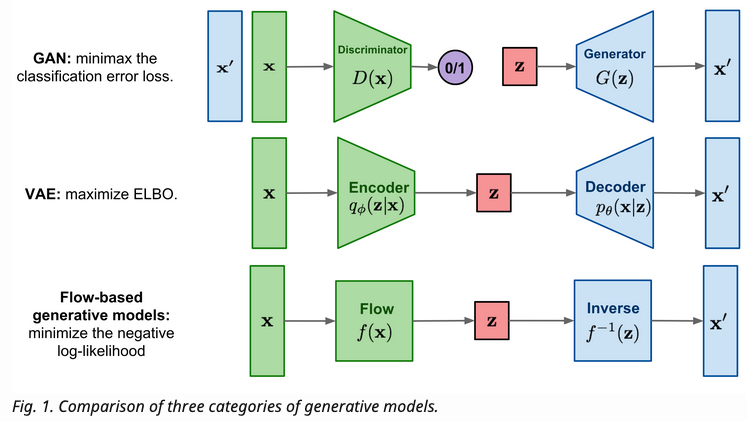
\includegraphics[width=\columnwidth]{GenerativeModels.png}
\caption{Different Generative Flows~\cite{weng2018flow}}
\label{fig:gens}
\end{figure}

\subsection{Normalizing Flows}
Normalizing Flows are unsupervised generative models that try to learn the exact
distribution of a dataset. It accomplishes this by use of change of variables.
This is defined as having a random variable $X$ with a probability density
function $f_X(x)$, where $x\in X$, we can calculate the probability density
function of some other variable $Z=g(x)$. In the case of normalizing flows we
use a prior probability distribution $p_Z$ on a latent variable $z\in Z$ and a
bijective function $f: X\mapsto Z$ (with $g = f^{-1}$ then we can find the
distribution on $X$ as
\begin{equation}
    p_X(x) = p_Z(f(x))\left | det\left(\frac{\partial f(x)}{\partial x^T}
        \right)\right |
\end{equation}
Commonly this is written with the log form for easier computation
\begin{equation}
    \log(p_X(x)) = \log(p_Z(f(x))) + \log\left(\left| det \left(
            \frac{\partial f(x)}{\partial x^T} \right) \right | \right )
\end{equation}
Where $\frac{\partial f(x)}{\partial x^T}$ is the Jacobian of $f$ at $x$. The
Jacobian is difficult to solve computationally and many works, such as the three
above, solve this by using LU decomposition. This makes it easier because that
creates a triangular matrix, where the determinant can be solved as the product
of the diagonal elements. 
\begin{equation}
    \frac{\partial f(x)}{\partial x^T} = \begin{bmatrix} I_d & 0 \\ \frac{\partial
    z_{I_2}}{\partial x_{I_2}} & \frac{\partial z_{I_2}}{\partial
    x_{I_2}}\end{bmatrix}
\end{equation}
By using LU decomposition this turns the computation from $\mathcal{O}(n^3)$ to
$\mathcal{O}(n)$~\cite{glow}.

This change of variables formula is what makes normalizing flows work. A
bijective function is used to learn from one probability distribution to
another, and the reverse. Figure~\ref{fig:nf} shows how bijective functions are
stacked together.

\begin{figure}[ht]
\center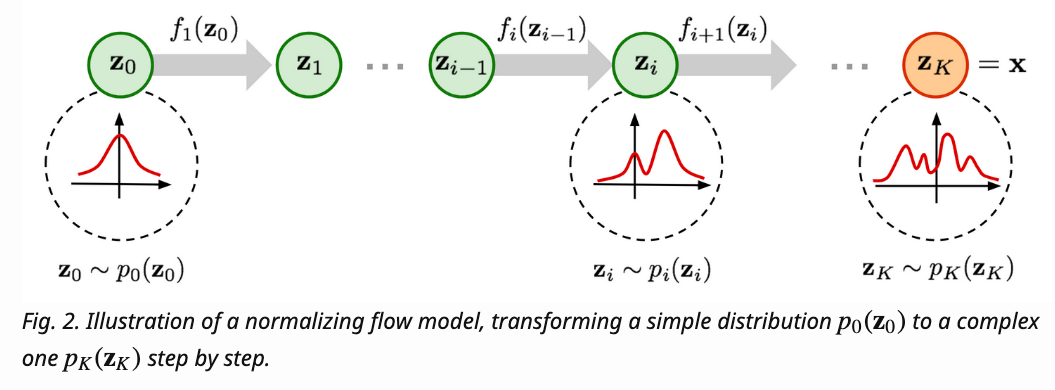
\includegraphics[width=\columnwidth]{NFs.png}
\caption{Flow Layers of Normalizing Flows~\cite{weng2018flow}}
\label{fig:nf}
\end{figure}

By stacking multiple bijective functions together one can think of it as
increasing the polynomial fit to the function. A common bijective function used
in normalizing flows is the simple linear equation $y = \sigma x + \mu$. This
function is easy to compute and trivially invertible. One step of flow results
in a polynomial fit of $x$ while $n$ steps of flow represents a polynomial fit
of $x^n$. 

These qualities make normalizing flows tractable and give it many benefits. The
problem with them is that they are more computationally expensive, compared to
models like GANs and VAEs, and requires significantly more data. Because
normalizing flows are learning the exact representation they need to more
learning examples, on the same order as the number of features that are being
learned~\cite{jainilecture}.
